\documentclass{article}
\usepackage{graphicx}
\usepackage{datetime}
\usepackage{geometry}
\usepackage{placeins}
\usepackage{minted}
\usepackage{xcolor}
\usepackage{caption}
\usepackage{lmodern} 
\usepackage[document]{ragged2e}
\usepackage[hidelinks]{hyperref}
\usepackage{enumitem}
\geometry{
 a4paper,
 left=25mm,
 top=25mm,
 }
\captionsetup{hypcap=false} 
\newdateformat{daymonthyear}{\THEDAY .\THEMONTH .\THEYEAR}
\title{
  \centering
  
\includegraphics[width=\textwidth]{images/logo_PWr_kolor_poziom.png}\\
  \fontsize{28pt}{30pt}\selectfont Sprawozdanie 7\\
  \fontsize{14pt}{30pt}\selectfont Ćwiczenie 7.Modemy. Transmisja sygnałów cyfrowych}
  \author{Krzysztof Zalewa,Wiktor Wojnar}
\date{\daymonthyear\today}
\renewcommand*\contentsname{Spis treści}
\renewcommand{\figurename}{Rysunek}
\renewcommand{\listingscaption}{Fragment kodu}
\begin{document}
    \maketitle
    \pagebreak
    \tableofcontents
    \FloatBarrier
    \section{Wstęp teoretyczny}
        \subsection{Metody konfiguracji modemów.}
            \subsubsection{Komendy Hayes}
                Komendy Hayes (zbiór komend AT) to specjalny język komend originalnie stworzony
                na potrzeby modemu firmy Hayes w 1981. Obecnie zbiór ten stał się standardem
                i jest używany w większości nowoczesnych urządzeń. Zbiór ten można podzielić na 
                cztery grupy:
                \begin{enumerate}
                    \item \textbf{Komendy podstawowe} - Duża litera i cyfra.Np I0.
                    \item \textbf{Komendy rozszerzone} - Znak \& ,duża litera i cyfra. Rozszerza podstawowy 
                        zbiór więc I0 != \&I0.
                    \item \textbf{Komendy własne} - Zwykle poprzedzone \textbackslash lub \%. Te komendy są 
                        bardzo różne ponieważ są pozostawione potrzebom producentów.
                    \item \textbf{Komendy rejestrów} - S n gdzie n to numer rejestru. Bezpośrednio modyfikuje
                        miejsce w pamięci urządzenia.
                \end{enumerate}
                \begin{table}
                    \begin{tabular}{|l|l|p{8cm}|}
                        \hline
                        Modem A & Modem B & Komentaż \\ \hline
                        ATDT12345678987 & & Użytkownik A podaje komendę do modemu A ATtention; D-Dial; T-Touch-Tone;
                        Zadzwoń na ten numer 12345678987 \\ \hline
                        & Dzwoni & Modem A rozpoczyna dzwonienie na modem B. Modem B daje znać o przychodzącym 
                        połączniu\\ \hline
                        & ATA & Komputer B odbiera połączenie\\ \hline
                        Połączenie & Połączenie & Oba modemy wyświetlają informację o poprawnym połączeniu.\\ \hline
                        qwerty & qwerty & Kiedy modemy są połączone\\ \hline
                        & +++ & Przejście do trybu poleceń\\ \hline
                        & OK & Potwierdzenie wykonania polecenia\\ \hline
                        & ATH & Komenda przerwania polecenia\\ \hline
                        Brak połączenia & OK & Potwierdzenie wykonania polecenia \\ \hline
                    \end{tabular}
                \end{table}
                \FloatBarrier
                \begin{figure}[ht]
                    \centering
                    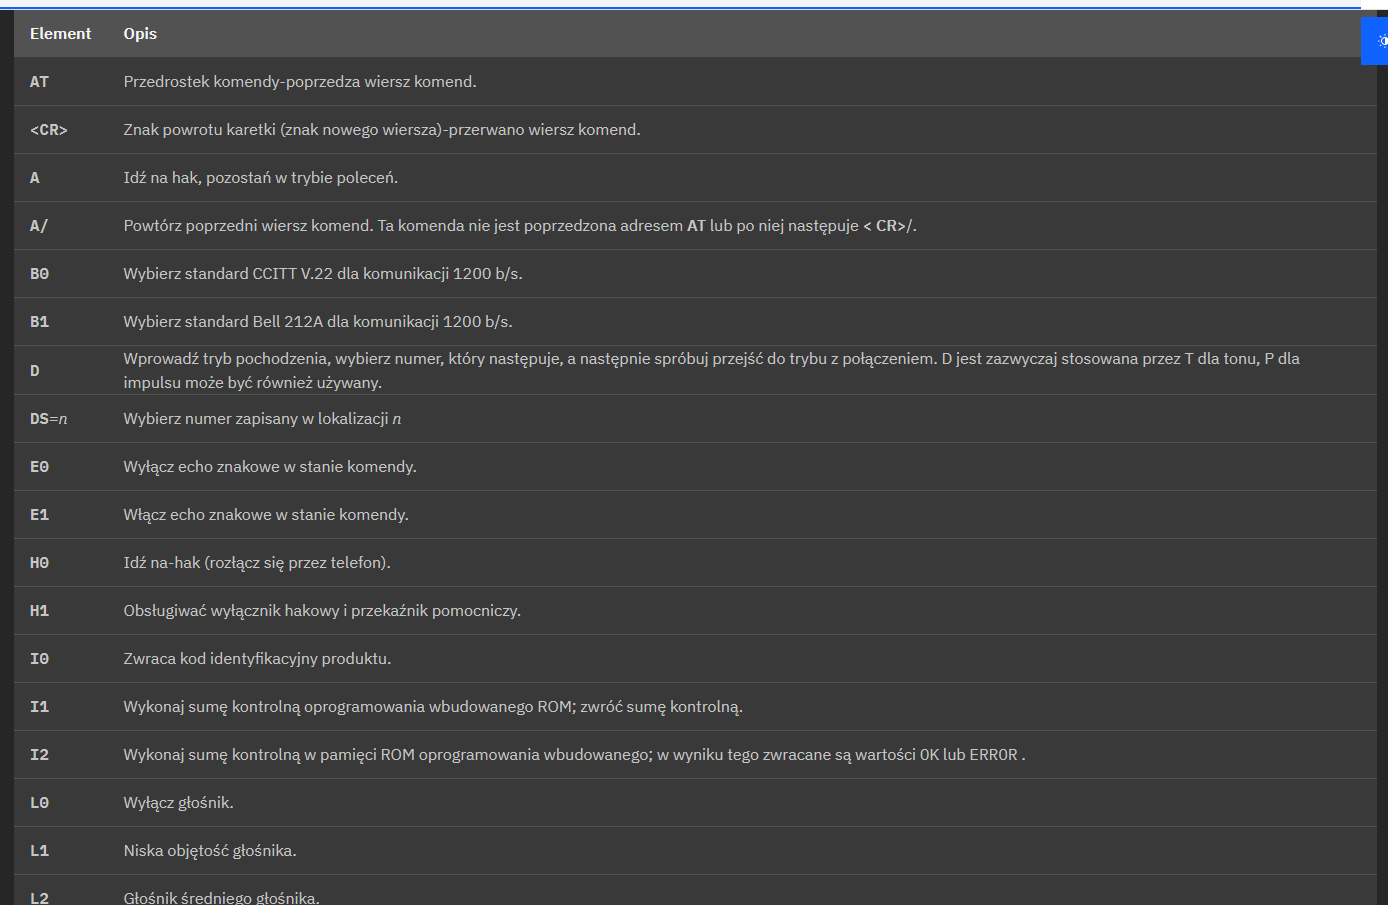
\includegraphics[width=\textwidth]{images/Zrzut ekranu 2025-02-02 214224.png}
                    \caption{Przykładowe komendy Hayes'a}
                    \label{fig:tex2}
                \end{figure}
                \FloatBarrier   
    \section{Zadanie laboratoryjne}
    \raggedright
        \subsection{Treść zadania}
            W ramach zajęć laboratoryjnych należało skonfigurować i przetestować połączenie 
            między dwoma modemami. Następnie należało napisać program który będzie w stanie
            wykonywać funkcje takie jak łączenie się z modemem, transmisja terminal-terminal
            oraz przesył plików.
        \subsection{Opis działania programu}
            Program może wykonywać jednocześnie role nadawcy i odbiorcy(Po wybraniu odpowiedniej 
            opcji). Po wybraniu opcji nadawania program łączy się z wybranym modemem (Modem 
            docelowy powinien być w trybie auto odbierania). Następnie można wybrać opcje 
            przesyłu plików lub teskstu. Po wybraniu trybu odbierania program oczekuje na 
            połączenie. Kiedy połączenie zostanie potwierdzone odbierane i wyświetlane są
            wiadomości z modemu 1.
        \subsection{Kod programu}
            \begin{frame}
                \scriptsize
                \inputminted[
                    style={vs},
                    breaklines,
                    breakanywhere, 
                    linenos, 
                    tabsize=4 
                ]{python}{Lab7.py}
                \vspace{1em}
                \captionof{listing}{Fragment kodu z programu}
                \label{lst:code}
            \end{frame}
    \section{Źródła}
        \begin{enumerate}[label=\arabic*.]
            \item \url{https://en.wikipedia.org/wiki/Hayes_AT_command_set}
            \item \url{https://www.ibm.com/docs/pl/aix/7.3?topic=troubleshooting-commands}
        \end{enumerate}
\end{document}